\documentclass{sigchi}

% Use this section to set the ACM copyright statement (e.g. for
% preprints).  Consult the conference website for the camera-ready
% copyright statement.

% Copyright
\CopyrightYear{2020}
%\setcopyright{acmcopyright}
\setcopyright{acmlicensed}
%\setcopyright{rightsretained}
%\setcopyright{usgov}
%\setcopyright{usgovmixed}
%\setcopyright{cagov}
%\setcopyright{cagovmixed}
% DOI
\doi{https://doi.org/10.1145/3313831.XXXXXXX}
% ISBN
\isbn{978-1-4503-6708-0/20/04}
%Conference
\conferenceinfo{CHI'20,}{April  25--30, 2020, Honolulu, HI, USA}
%Price
\acmPrice{\$15.00}

% Use this command to override the default ACM copyright statement
% (e.g. for preprints).  Consult the conference website for the
% camera-ready copyright statement.

%% HOW TO OVERRIDE THE DEFAULT COPYRIGHT STRIP --
%% Please note you need to make sure the copy for your specific
%% license is used here!
% \toappear{
% Permission to make digital or hard copies of all or part of this work
% for personal or classroom use is granted without fee provided that
% copies are not made or distributed for profit or commercial advantage
% and that copies bear this notice and the full citation on the first
% page. Copyrights for components of this work owned by others than ACM
% must be honored. Abstracting with credit is permitted. To copy
% otherwise, or republish, to post on servers or to redistribute to
% lists, requires prior specific permission and/or a fee. Request
% permissions from \href{mailto:Permissions@acm.org}{Permissions@acm.org}. \\
% \emph{CHI '16},  May 07--12, 2016, San Jose, CA, USA \\
% ACM xxx-x-xxxx-xxxx-x/xx/xx\ldots \$15.00 \\
% DOI: \url{http://dx.doi.org/xx.xxxx/xxxxxxx.xxxxxxx}
% }

% Arabic page numbers for submission.  Remove this line to eliminate
% page numbers for the camera ready copy
% \pagenumbering{arabic}

% Load basic packages
\usepackage{balance}       % to better equalize the last page
\usepackage{graphics}      % for EPS, load graphicx instead 
\usepackage[T1]{fontenc}   % for umlauts and other diaeresis
\usepackage{txfonts}
\usepackage{mathptmx}
\usepackage[pdflang={en-US},pdftex]{hyperref}
\usepackage{color}
\usepackage{booktabs}
\usepackage{textcomp}
\usepackage{float}

% Some optional stuff you might like/need.
\usepackage{microtype}        % Improved Tracking and Kerning
% \usepackage[all]{hypcap}    % Fixes bug in hyperref caption linking
\usepackage{ccicons}          % Cite your images correctly!
% \usepackage[utf8]{inputenc} % for a UTF8 editor only

% If you want to use todo notes, marginpars etc. during creation of
% your draft document, you have to enable the "chi_draft" option for
% the document class. To do this, change the very first line to:
% "\documentclass[chi_draft]{sigchi}". You can then place todo notes
% by using the "\todo{...}"  command. Make sure to disable the draft
% option again before submitting your final document.
\usepackage{todonotes}

% Paper metadata (use plain text, for PDF inclusion and later
% re-using, if desired).  Use \emtpyauthor when submitting for review
% so you remain anonymous.
\def\plaintitle{An evaluation of TRIO’s e-learning module enhancing the communication between cancer patients, clinicians and caregivers}
\def\plainauthor{First Author}
\def\emptyauthor{}
\def\plainkeywords{Authors' choice; of terms; separated; by
  semicolons; include commas, within terms only; this section is required.}
\def\plaingeneralterms{Documentation, Standardization}

% llt: Define a global style for URLs, rather that the default one
\makeatletter
\def\url@leostyle{%
  \@ifundefined{selectfont}{
    \def\UrlFont{\sf}
  }{
    \def\UrlFont{\small\bf\ttfamily}
  }}
\makeatother
\urlstyle{leo}

% To make various LaTeX processors do the right thing with page size.
\def\pprw{8.5in}
\def\pprh{11in}
\special{papersize=\pprw,\pprh}
\setlength{\paperwidth}{\pprw}
\setlength{\paperheight}{\pprh}
\setlength{\pdfpagewidth}{\pprw}
\setlength{\pdfpageheight}{\pprh}

% Make sure hyperref comes last of your loaded packages, to give it a
% fighting chance of not being over-written, since its job is to
% redefine many LaTeX commands.
\definecolor{linkColor}{RGB}{6,125,233}
\hypersetup{%
  pdftitle={\plaintitle},
% Use \plainauthor for final version.
%  pdfauthor={\plainauthor},
  pdfauthor={\emptyauthor},
  pdfkeywords={\plainkeywords},
  pdfdisplaydoctitle=true, % For Accessibility
  bookmarksnumbered,
  pdfstartview={FitH},
  colorlinks,
  citecolor=black,
  filecolor=black,
  linkcolor=black,
  urlcolor=linkColor,
  breaklinks=true,
  hypertexnames=false
}

% create a shortcut to typeset table headings
% \newcommand\tabhead[1]{\small\textbf{#1}}

% End of preamble. Here it comes the document.
\begin{document}

\title{\plaintitle}

\numberofauthors{1}
\author{%
  \alignauthor{Melanie Bonnaudet\\
    \affaddr{The University of Sydney}\\
    \affaddr{Sydney, Australia}\\
    \email{melbon@kth.se}}\\
}

\maketitle

\begin{abstract}
 150 words. The abstract should be a concise statement of the problem, approach, and conclusions of the work described. It should clearly state the paper's contribution to the field of HCI\@.
\end{abstract}


% ACM Classfication

\begin{CCSXML}
<ccs2012>
<concept>
<concept_id>10003120.10003121</concept_id>
<concept_desc>Human-centered computing~Human computer interaction (HCI)</concept_desc>
<concept_significance>500</concept_significance>
</concept>
<concept>
<concept_id>10003120.10003121.10003125.10011752</concept_id>
<concept_desc>Human-centered computing~Haptic devices</concept_desc>
<concept_significance>300</concept_significance>
</concept>
<concept>
<concept_id>10003120.10003121.10003122.10003334</concept_id>
<concept_desc>Human-centered computing~User studies</concept_desc>
<concept_significance>100</concept_significance>
</concept>
</ccs2012>
\end{CCSXML}

\ccsdesc[500]{Human-centered computing~Human computer interaction (HCI)}
\ccsdesc[300]{Human-centered computing~Haptic devices}
\ccsdesc[100]{Human-centered computing~User studies}

% Author Keywords
\keywords{\plainkeywords}

% Print the classficiation codes
\printccsdesc
Please use the 2012 Classifiers and see this link to embed them in the text: \url{https://dl.acm.org/ccs/ccs_flat.cfm}


\section{Introduction}

Cancer incidences are rising and becoming overall more common, according to Bray. F. et al.’s global cancer statistics 2018 \cite{Bray2018}. As it affects millions of people across the world it is important to provide the best cancer care as possible.

The cancer patient’s medical situation and decisions has impact on its relatives’ life and health \cite{Bevans2012}. Therefore, it is important that relatives are able to participate in the patient’s medical consultations and decision making. It has not always been the case that relatives have been aloud to participate [\textbf{reference}]. Each patient should have one main caregiver that can accompany and support the patient. The caregiver and relatives have expressed needs in medical and behavioural information \cite{Lamore2017}. Oncologists also revealed needs to learn how to provide adapted information for caregivers \cite{Stuij2018}. For an ideal cancer care, patients, caregivers and oncologists need to enhance their communication and behavioural skills for medical situations. 

\textit{"TRIO, Clinician-patient-family working together for quality care"} is based on a TRIO Framework, introduced by Laidsaar-Powell, R. et al. \cite{Laidsaar-Powell2017}. It is constituted of three main persons:

\begin{itemize}
    \item The \textbf{cancer patient}: refers to a cognitively competent adult cancer patient.
    \item The \textbf{main clinician}: usually an oncology physician.
    \item The \textbf{main caregiver}: usually accompanying the patient to medical consultations and assisting in the patient’s care. The caregiver is related to the patient biologically, legally or emotionally.
\end{itemize}

To enhance the communication between cancer patients, their caregivers and oncologists, the TRIO project has created an online learning platform. Each group has its own learning platform with learning modules covering different topics. It is a multimedia e-learning platform as it is constituted of text, videos and different interactive activities. These are, for example, yes-no questions, sorting cards according to their importance, surveys about the user’s emotional profile, etc. This type of content makes learning an active process but inadequate user experience can affect the learning outcome negatively \cite{Huang2005}. Therefore, this study aims to evaluate the usability and use of TRIO.

\section{Background}
Laidsaar-Powell, R. et al. ~\cite{Laidsaar-Powell2017} introduced the notion of a TRIO Framework, also called TRIO Triangle. As shown in figure 1, it is constituted of a cancer patient, a main clinician and a main caregiver. The purpose was to study why it is important to understand the  involvement of family caregivers in cancer care. Their study shows to which extent they are involved in treatment decisions in cancer consultations. Results have proven that caregivers’ involvement depend on several factors and vary from person to person. These factors can be demographic, psychological, relational, cultural and medical. Three different cases are given with different influences in decision making from the caregiver.

First case, a patient and oncologist discuss whether to undergo chemotherapy or not. The caregiver states they will support whatever decision the patient takes. As shown in figure 1, the decision is focused between the patient and oncologist.

\begin{figure}[H]
\centering
  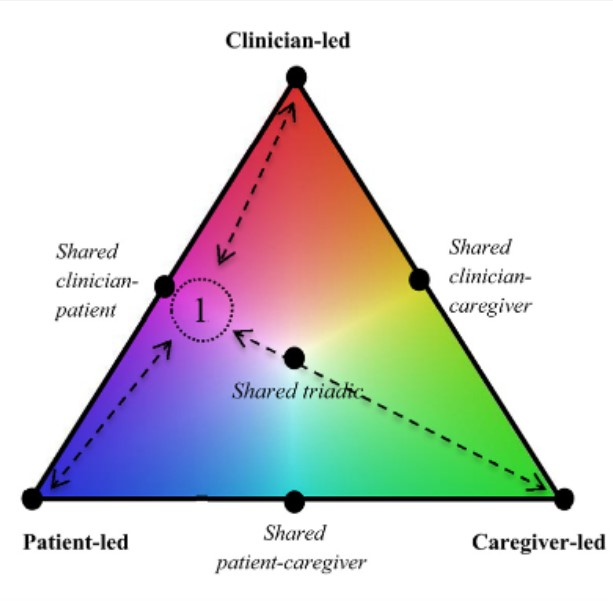
\includegraphics[width=0.9\columnwidth]{figures/Triangle1Screenshot.jpg}
  \caption{TRIO Framework/Triangle with focus between the patient and the clinician. Figure from}~\label{fig:figure1}
\end{figure}

Second case, a patient has to choose whether to delay chemotherapy or to undergo fertility treatment. The patient discusses this with her husband, and he states he would prefer the fertility treatment for her and their family. As shown in figure 2, the decision-making focus is mainly on the patient followed by her husband.

\begin{figure}[H]
\centering
  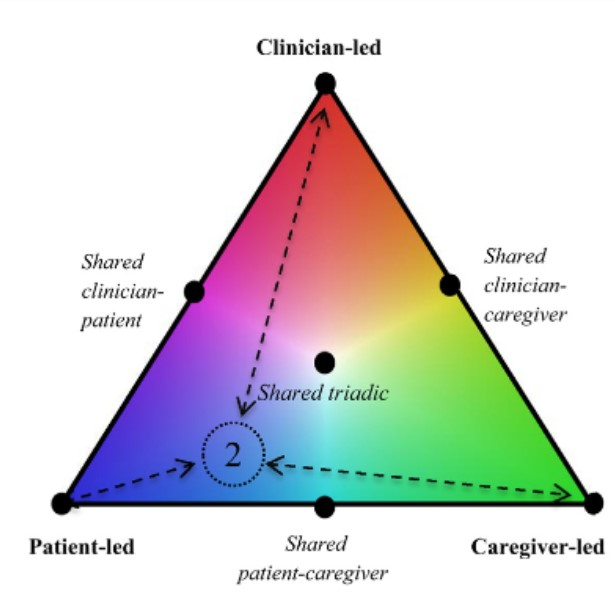
\includegraphics[width=0.9\columnwidth]{figures/Triangle2Screenshotjpg.jpg}
  \caption{TRIO Framework/Triangle with focus between the patient and the caregiver. Figure from}~\label{fig:figure1}
\end{figure}

Third case, a patient with limited English proficiency has cancer and his son, fluent in English, exchanges all information with the oncologist. The son directs the conversation with consent of the patient. As shown in figure 3, the decision-making focus relies on the son, the caregiver.

\begin{figure}[H]
\centering
  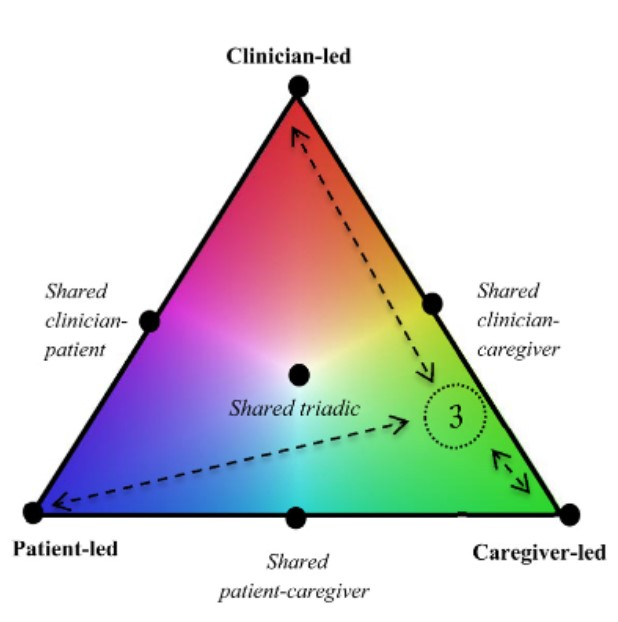
\includegraphics[width=0.9\columnwidth]{figures/Triangle3Screenshot.jpg}
  \caption{TRIO Framework/Triangle with focus between the clinician and the caregiver. Figure from}~\label{fig:figure1}
\end{figure}

Knowing how much each party is involved is important for TRIO’s e-learning platform as all three are targets groups for the website. 

Ruiz, J. G. et al. ~\cite{Ruiz2006} have studied e-learnings’ effectiveness and how it fits into the medical world. E-learning enhances individual’s individual learning. It can be integrated into education as well as be used during duty hours. Being able to use e-learning in these circumstances, is very convenient for the medical world. The study also points out important things to think about when evaluating an e-learning platform such as the ease of use, navigation, the material, interaction, etc. Without those the e-learning loses its effectiveness. Therefore, the TRIO e-learning is very suitable for its user groups, if the usability is adequate. 

The first steps in how to develop an e-learning platform for oncologists to improve their information-giving skills has been studied by Stuij S. M. et al. ~\cite{Stuij2018}. They have shown the oncologist’s learning needs within how they should provide information to patients as well as their training preferences within their profession. Oncologist desire to be able to adapt the information for patients, structure the information and deal with patient’s emotions. Focus groups and interviews revealed that the preferred learning method is a digital platform with multimedia content such as videos. Feedback from peers, experts and patients would also be appreciated. They want to be able to adapt their learning to their own personal needs, have it easily accessible and simple of use. The TRIO platform fulfills these needs by letting the user choose which module they want to do without having to follow a particular order, and can complete them whenever they want to. 

What roles family members have in the decision-making of treatment for people with chronic diseases has been studied by Lamore, K. et al. ~\cite{Lamore2017}. Family members need to be provided with medical knowledge and often want to participate in decision-making discussions. For this, they must have helpful behaviours, not being dominating, providing information and support the patient. The patient must also decide when they need a private conversation with the physician. This study mentions all three parties are positive towards the involvement of caregivers in medical consultations and decisions. Although, for this to work well caregivers need information, both medical and behavioural. The TRIO website has this aim which is why it is important to study the platform before being released for an optimal learning and caregiver involvement. 

How the partner’s involvement is related to decision making in triad cancer consultations has been studied by Bracher, M. ~\cite{Bracher2019}. In these consultations the partner has had different roles, behaviours and relationships with patient and physician. Some have been dominant, interruptive, refusing to cede while other characteristics have been emotional support, helpful contributions such as self-initiated questions. Spouses and children are more likely to engage than relatives and friends. Some physicians interacted more with the patient than the partner and often shift back the conversation to the patient. This shows how all involved in triad consultations need to get a better understanding of their role and communication with each other.

A review of research on the health of the caregiver and the patient by Hodges, L. J. et al. ~\cite{Hodges2005} showed there is an association between their well-being. The caregiver’s psychological health and stress level is strongly related to the partner’s health and stress. The patient is very likely to become distressed when their carer does, they then become a similar level of distress. Bevans, M. et al. ~\cite{Bevans2012} have studied how a caregiver’s life and health get influenced by the care-giving responsibilities of a cancer patient. These responsibilities bring stress and burdens that affect the caregiver negatively. Stressful moments are inevitable, but they can be eased. Avoiding barriers between caregivers and physicians by letting caregivers participate in the medical proceedings, is a good prevention. McCarthy, B. ~\cite{McCarthy2011} has studied carers’ information needs. They need information and often want to hear it from the physicians. Often, they have to actively seek it from physicians and can feel ignored. Cases where carers are content with the communication had met their informational needs. This shows how communication is important for everyone’s well-being. The TRIO website has an important aim to fix these issues.  

Huang, C. ~\cite{Huang2005} shows that designing an interactive multimedia learning tool gives it dynamic content interactive with, which makes learning an active process. Other features to enhance this, is to be able to immediately test your knowledge and easily visualise information. Several steps are recommended to create such a tool. It is needed to understand the learning goal and the user needs to then design the content and utilize adequate technology. Multimedia materials need to be created with website standards and consider human factors. User tests are then required to be able to evaluate and improve the design. Recommended questions to think of are:

\begin{itemize}
    \item what they will learn, 
    \item why would they want to learn this, 
    \item what they can do on the page and get feedback on how they are doing. 
\end{itemize}

When the module is built, user tests and heuristic evaluation are needed to know how the modules perform. Technical problems can interfere with the learning outcome. Science, education and technology knowledge must be combined for an excellent educational media. The current state of the TRIO website is that it needs to be evaluated to get its best user experience which will be reported in this study. 

Briz-Ponce, L. ~\cite{Briz-Ponce2017} show that most student participants of the study own a mobile device and that mobile technologies are constantly increasing. Medical students are positive towards mobile learning and recommending it. However, their willingness of use is only medium high as they had a low ease of use perception of mobile learning. This shows how important it is for a mobile learning platform to provide a good user experience. The TRIO website is available on mobile and should therefore be tested with its users. 



\section{Method}
this is how 

\section{Results}
results

\section{Discussion}
discuss

\section{Conclusion}
test~\cite{Laidsaar-Powell2017}

\section{Acknowledgments}

% BALANCE COLUMNS
\balance{}

% REFERENCES FORMAT
% References must be the same font size as other body text.
\bibliographystyle{SIGCHI-Reference-Format}
\bibliography{MasterThesis}

\end{document}

%%% Local Variables:
%%% mode: latex
%%% TeX-master: t
%%% End:
